\documentclass[a4paper,man,natbib]{apa6}
%\usepackage[square]{natbib}
\usepackage{microtype}
\usepackage{mathtools} % needed
\usepackage{hyperref}
%\usepackage{stmaryrd} % not needed
\usepackage{tabularx}
\usepackage[normalem]{ulem}
%\linespread{1.3}
% use apa defaults
\hypersetup{hidelinks=true}
% let's not be garish

\newcommand*{\smex}[1]{\textit{#1}} % 'small example'
\newcommand*{\spex}[1]{``{#1}''} % 'spoken example'
\newcommand*{\term}[1]{\emph{#1}} % introducing a new term
\newcommand*{\citegen}[1]{\citeauthor{#1}'s \citeyear{#1}}


\title{Contextual effects on online pragmatic inferences.}
\author{JK; JL; MC}
\date{\today}


\shorttitle{disfluency|distraction}
\abstract{Where the veracity of a statement is in question, listeners show a bias towards interpreting speaker disfluency as a sign of dishonesty. 
This bias is not limited to post-hoc judgements, but can also be found during online speech processing. 
The present study investigates whether listeners are influenced by contextual information about the potential causes of speaker disfluency. 
If listeners make inferences about the cause of a disfluency, then a plausible speaker-distraction may attenuate the inclination to interpret an utterance as dishonest.

Participants listened to a speaker describe the locations of treasure (``The treasure is behind [the]/[thee---uh---] \textless referent\textgreater .''), while viewing scenes comprising the referent and a distractor. 
They were told that not all utterances would be honest, and their task was to click on the suspected location of the treasure. 
In line with previous work, participants were more likely to click on the distractor when the description was disfluent, and this effect corresponded to an early fixation bias, demonstrating the online nature of the pragmatic judgement.

The present study, however, also manipulated the presence of a plausible external cause of speaker disfluency. 
To accomplish this, participants were told that all utterances were produced outside on a busy street, and all items were played over low-level ambient street noise.

When there was a plausible external cause of the speaker disfluency (a distracting noise, in the form of a car-horn), participants were more likely to initially fixate on the referent, only later fixating on and selecting the distractor. 
One account of these findings would suggest that participants made early inferences about the contextual causes of disfluencies, which were eventually overridden by a dishonesty bias for disfluent utterances.}


\begin{document}
\maketitle


\section{Background}
Everyday speech is for the most part spontaneous, and thus often disfluent, containing pauses, \spex{um}s, \spex{uh}s, repetitions, revisions, and mispronunciations.
Excluding silent pauses, naturally occurring speech has a rate of approximately~6 to~10 disfluencies per~100 words \citep{Bortfeld2001,FoxTree1995}.
The disfluent nature of speech is just one of many variable aspects of \emph{how} an utterance might be presented, and listeners must be able to cope with this variability in order to successfully understand a speaker.

Disfluencies in speech are not merely incidental.  Speakers are more disfluent when utterance planning involves low-frequency words \citep{Beattie1979}, less-preferred syntactic structures \citep{Cook2009}, discourse-new expressions \citep{arnold2000heaviness}, or a greater choice of expressive alternatives \citep{Schachter1991}.
In this way, disfluencies provide paralinguistic `cues' about the content of a speaker's message.
Research has shown that listeners can, and do, exploit these cues to make predictions about upcoming speech.
For example, following a disfluency, they are more likely to predict the introduction of a new object into the discourse, as shown by visual world eye movements \citep{Arnold2004}, and less likely to have difficulty integrating an unpredictable word into its context, as indexed by a reduction in the N400~ERP component \citep{Corley2007}.

Evidence from a series of eyetracking experiments suggests that predictions like these are sensitive to context.
\citet{Arnold2007} asked participants to click on depictions of easy-to-name (ice-cream) or harder-to-name (abstract symbol) items in response to auditory instructions.
Where the instructions were disfluent, participants were more likely to fixate harder-to-name items before they heard the item name.
Importantly, these fixation biases were modulated when participants were told that the speaker had object agnosia, and hence might be presumed to have difficulty naming easy-to-name items.
The fact that a prediction that a hard-to-name item will follow a disfluency can be modulated by contextual information suggests that on encountering a disfluency, participants are not merely making a stochastic prediction about what might be mentioned next.
Instead, they may be actively modelling the speaker in order to account for the disfluency encountered and make situation-specific predictions.

However, the picture is far less clear when the cause of the disfluency is local, in the sense that it could be assumed to be the cause of a specific instance of disfluency, rather than of a heightened probability of disfluency in general.
In \citeauthor{Arnold2007}'s Experiment~3, for example, local causes (beeps and construction noises, assumed to distract the speaker momentarily) did not affect listeners' biases to fixate harder-to-name objects following disfluency.
Moreover, several studies have shown that listeners do not seem especially sensitive to the nature of the disfluency:  They have been shown to be affected by dog barks \citep{bailey2003disfluencies} and sine waves \citep{corley2011helps} when they are substituted for filled-pause disfluencies.
This sensitivity to non-linguistic interruptions sits poorly with the idea that the listener is modelling the speaker's production system, to anything greater than a superficial extent.

One reason that it is hard to conclude about what is being modelled is that, in the studies outlined above, the effects of disfluency are ephemeral.
Disfluency might affect what listeners think they are about to hear, but it has no lasting consequences at the message level:
The fluent and disfluent versions of the utterances used mean the `same thing'.
For that reason, the consequences to the listener of mismodelling the speaker are trivial, and the behavioural consequences of any such modelling relatively hard to detect.
However, a parallel literature shows that in some circumstances, disfluency has pragmatic effects, in that it has direct consequences for the way a listener interprets an utterance.
%
%FO(A)K; other pragmatics; lying; Jia \ra{}question:  Now we're talking about \emph{pragmatic} effects, is there evidence of speaker modelling?
For example, \citet{Brennan1995} based their comprehension study on evidence that speakers use disfluency to manage difficulty in retrieving information \citep{Smith1993}.
Participants were played recordings of answers to general knowledge questions which had been obtained during a production study.
The answers were digitally edited and were sometimes preceded by either a silent pause, or a filler.
Listeners rated the answers as being less likely to be correct when the recorded answers were preceded by silence or fillers.
In other words, their interpretations of, rather than simply predictions concerning, the utterances they heard were directly affected by disfluency \citep[see also][]{Swerts2005}.
Listeners faced with disfluency had less confidence in the speaker's knowledge (a weaker ``Feeling of Another's Knowing'', or FOAK), and therefore revised their estimates concerning the factual correctness of what was being said.

%%% NB I couldn't find much evidence of "other pragmatic" effects.  I
%%% do seem to recall some social psych papers talking about
%%% disfluency as hedging; would be great if we could find those

As well as producing statements about which they have little confidence, speakers can easily utter propositions which they know to be false.
This form of lying \citep[see][for another]{frankfurt05} is often thought to be associated with cognitive effort.
According to this view, the increased load involved in formulating and uttering a lie may lead speakers to provide verbal and non-verbal cues to deception, including disfluency \citep{Zuckerman1981,depaulo2003cues}.
Listeners' interpretations appear to reflect such this hypothesis:
\citet{Zuckerman1981} found hesitations in speech to be reliably associated with a perception of dishonesty, in both judgments made by speakers about themselves, and judgments made about another speaker.
%%%%%%%% need link here. importance is comp not produ.
%%%% DOES THIS FLOW?

In both FOAK and lying research, the proposed mechanism by which the interpretation of what is said is affected by disfluency is via \term{speaker modelling}:
By reverse inference, disfluency is a symptom of cognitive difficulty, and cognitive difficulty is the consequence of limited knowledge (FOAK) or of inventing a situation (lying).
In other words, to conclude that the speaker is lying requires reasoning about his or her cognitive state, in line with earlier claims by \citet{Arnold2007}.
However, listeners may in fact not reason in this way.
Instead, they may heuristically associate certain aspects of spoken performance with uncertainty or lying, perhaps based on previous co-occurrence, or a superficial model of the speaker.
This heuristic association would only be affected by very clear evidence that it wasn't relevant.

% In disfluency research, the research questions concerning comprehension are driven by a view of the regularities that might exist in spoken language.
% The consequence of describing a hard-to-name object (prediction), limited knowledge (FOAK), or of inventing a situation (deception) is cognitive difficulty in formulating an utterance; and the consequence of cognitive difficulty is disfluency.
% Studies then test whether listeners are sensitive to disfluency in appropriate circumstances.
% What has remained 


One reason for believing that the association between disfluency and lying is heuristically calculated is evidence from \citet{Loy2016}, which highlights the speed at which pragmatic interpretations are made.
\citeauthor{Loy2016}'s study was framed as a treasure hunting game, in which listeners were asked to guess the location of a reward by clicking on one of two depicted objects in each trial.
Participants heard recorded utterances which indicated the location of the treasure, and which were either fluent or disfluent (\spex{The treasure is behind [the]/[thee---uh---] \textless referent\textgreater}).
Participants were told that the speaker would be dishonest half of the time. 
The judgements which participants made about the speaker's honesty in each trial were implictly measured by examining which of the two objects they clicked:
Clicking on the named object corresponded to a judgement that the speaker was telling the truth, whereas a click on the other object meant that the speaker was thought to be lying.
In line with previous research linking disfluency to deception \citep{Zuckerman1981},  participants were less likely to click on the named object following disfluent utterances (and instead, tended to click on the object which had not been mentioned).
Importantly, eye- and mouse-tracking records showed that this effect emerged as soon as it became clear which of the two objects was being named:
In other words, participants' pragmatic judgements were shown to be influenced by disfluency at the earliest detectable moment.
If detailed speaker modelling is occurring, any inferences regarding the cause of a given disfluency would have to be made very fast.

%%% so this becomes another reason for assuming that it's a heuristic????
%%%%%%%%%%%%%%%%%%%%%%%%%%%%%%%%%%%%%%%%%%%%%%%%%%%%%%%%%%%%%%%%%%%%%%%%%
Another reason for assuming that a heuristic is at play is that listeners' interpretations of disfluency may be inaccurate.
Although listeners tend to associate disfluency with lying \citep{Loy2016,Zuckerman1981}, some evidence suggests that, in production, disfluency occurs more frequently during truth-telling than during deception \citep{Arciuli2010markers,Arciuli2009lies,Benus2006pauses}.
\citet{DePaulo1982actual} demonstrated a  mismatch between disfluency as an actual and as a perceived cue to deception:
The rates of filled pauses produced by speakers did not differ during descriptions they made about people whom they liked or disliked from descriptions made when they were asked to pretend to feel the opposite way about them. 
However, when listening to the descriptions made by other participants, higher rates of filled pauses were associated with an interpretation that the speaker was being deceitful \citep[see also][]{loy2016lying}.

%%% DELETEME
\fbox{please check this para}
%%% DELETEME
The evidence cited above suggests that, at least for the case of deception, the influence of speaker disfluency is fast, and not always accurate: 
Listeners appear to rely on a rule-of-thumb association between disfluency and lying.
However, it is possible that any inaccuracy is actually the result of a more detailed attempt to model the speaker.
Lying is associated with cognitive effort, and cognitive effort is associated with disfluency, predicated on not on experience as a listener but on introspection as a speaker:
Speakers believe themselves to be more disfluent when lying \citep{Zuckerman1981}, and this belief extends to others' language production.
Evidence for this conjecture would lie in whether listeners' assessments of speaker veracity were affected by specific circumstances which a heuristic would be unlikely to take into account.
One such circumstance would be the availability of an alternative cause of a given disfluency, such as speaker distraction.
If listeners are reasoning about the causes of speakers' disfluencies, and alternative causes of those disfluencies are readily available, then the association between disfluency and lying should be weakened.

In the current study, we build  \citegen{Loy2016} treasure hunting game, using an auditory context which provides plausible causes of speaker distraction (and thus disfluency).
Utterances are presented to listeners under the guise of having been recorded outdoors in a busy street, and low-level ambient noise is present behind every utterance.
In the critical condition, disfluencies are immediately preceded by relatively loud noises (here, car-horns).
If listeners rely upon a simple heuristic association between disfluency and deception, then the car-horn should not influence the judgments they make about a speaker's honesty.
If however listeners actively model a speaker by reasoning about the causes of specific disfluencies, the association between disfluency and deception should be weakened when the car-horn is present:
Listeners might attribute disfluency to the speaker being momentarily distracted, rather than to the intention to lie.


\section{Experiment}

The present experiment followed a 2 (fluent vs disfluent) x 2 (distraction absent vs present) design.
Subjects participated in a visual world paradigm game, similar to that
used by \citet{Loy2016}, in which they guessed the location of some treasure based on utterances made by a potentially deceitful speaker, ostensibly recorded outdoors in a busy street.
Half of the critical utterances were fluent, and half disfluent; in half of all critical cases, a car-horn was clearly audible immediately prior to the disfluency, or in the equivalent parts of fluent utterances.
As in \citet{Loy2016}, we measured eye- and mouse- movements, to study the time course of listeners' pragmatic judgments about the honesty of an utterance, as well as their final interpretation of each utterance (object clicked).


\subsection{Materials}
%\subsubsection{visual}
Visual stimuli consisting of 120 black and white line drawings, taken from \citet{Snodgrass1980}, were presented to participants in pairs across 60 trials (20 experimental, 40 fillers). 
Each trial presented the \textit{referent} (the object which the speaker identified as having the treasure behind for that trial), and a \textit{distractor}, which was chosen at random without replacement from a set of 60 objects. 
To control for the effect of the bias towards interpreting disfluency to difficulty of description \citep{Arnold2007}, critical referents and distractors were matched for familiarity (H value $\ge 3.0$) and ease-of-naming ($<1.0$). 
Object pairings with the same phonetic onset were avoided. 

%\subsubsection{utterances|audio}
As in \citet{Loy2016} each referent was associated with a recording of a speaker naming the depicted object as the location of the treasure, and as before, critical utterances were either fluent or disfluent. 
The present study, however, manipulated not only the manner of delivery, but also the presence of a plausible cause of speaker distraction. 
Thus audio files were constructed such that the critical referents could be heard in four conditions varying by delivery (fluent vs disfluent) and presence of distraction (absent vs present), see below. 
The disfluent variants were created by splicing a prolonged article followed by a filled pause (\spex{Thee---uh,}) into the fluent utterances.
Where \citet{Loy2016} studied both utterance-initial and utterance-medial disfluencies, we opted for an utterance-medial position as it was considered more believable as being caused by speaker distraction when paired with a environmental cue.
Meanwhile, to create a plausible cause of speaker-distraction, a 520ms car-horn sound effect was presented prior to the onset of the referent noun (-1100ms for disfluent utterances, -600ms for fluent). 
To situate the car-horn sound effect in a context, each referent was paired with a unique clip of ambient traffic and street noise, over which the recordings in their vario were presented.
Thus the presentation of each critical referent varied only by 1) fluency and 2) presence of car-horn, to ensure that participants' behaviour was a reaction to the different combinations of these elements. 
All recordings, ambient noise and sound-effects were normalised and resampled to create 48 KHz stereo .wav files.


\begin{enumerate}
\item \textbf{fluent, distraction absent:} The treasure is behind the \textless referent\textgreater .
\item \textbf{disfluent, distraction absent:} The treasure is behind thee, uh ... \textless referent\textgreater .
\item \textbf{fluent, distraction present:} The treasure is $\underbracket{\text{behind the}}_\text{horn}$ \textless referent\textgreater .
\item \textbf{disfluent, distraction present:} The treasure is $\underbracket{\text{behind thee}}_\text{horn}$, uh ...\textless referent\textgreater .
\end{enumerate}


%\subsubsection{lists}
The 20 critical referents were counterbalanced across four lists, each with 10 fluent and 10 disfluent utterances, and each containing 10 instances of the car-horn (5 of which were disfluent). 
Lists also contained 40 filler utterances, half of which were fluent, and half of which contained either a form of disfluency or a discourse manipulation (see Table \ref{table:fillers}). 
Additionally, 20 of these filler items (10 fluent, 10 disfluent or discourse manipulation) contained various novel noises which could be interpreted as distracting for a speaker (see Table \ref{table:fillernoise}). 
These filler distractions varied in position relative to the referent noun onset.

\begin{table}
\begin{tabularx}{\linewidth}{|X|X|X|X|}
  \hline
Filler type & Manipulation & No. of Utterances & Example \\
  \hline
Fluent & None & 20 & The treasure is behind the \textless referent\textgreater . \\
Disfluent & Prolongation & 3 & The treasure is behind \textit{thee...} \textless referent\textgreater . \\
& Repetition & 4 & The treasure is behind \textit{the- the} \textless referent\textgreater .\\
& Filled pause (utterance-inital) & 3 & \textit{Umm..} The treasure is behind the \textless referent\textgreater .\\
Other & Discourse marker & 5 & \textit{Okay,} the treasure is behind the \textless referent\textgreater .\\
& Modal & 3 & The treasure \textit{could be} behind the \textless referent\textgreater .\\ 
& Combination & 2 & \textit{Right,} the treasure \textit{might be} behind the \textless referent\textgreater .\\
   \hline
\end{tabularx}
\caption{Disfluencies and discourse manipulations in filler items.}
\label{table:fillers}
\end{table}

\begin{table}
\begin{tabularx}{\linewidth}{|X|X|}
\hline
Noise & No. of Utterances\\
\hline
Vehicle horns (various) & 7 \\
Sirens (various) & 3 \\
Vehicles revving (various) & 2 \\
Car-stereo & 2 \\
Bicycle-bell & 1 \\
Bus doors opening & 1 \\
Footsteps & 1 \\
Loose drain cover & 1 \\
Man shouting & 1 \\
Dog barking & 1 \\
\hline
\end{tabularx}
\caption{Plausible causes of speaker distraction in filler items.}
\label{table:fillernoise}
\end{table}


\subsection{Cover story}
Central to the idea of a distraction-caused-disfluency is the requirement that participants believe that the utterances were produced naturally and in a noisy environment. 
Participants were told that the recordings were made by a participant of a previous experiment which was conducted on the side of a busy street. 
To corroborate this, during the initial explanation of the experiment, participants were shown three videos claimed to be examples of the speaker producing the utterances. 
These were presented alongside the images about which the speaker spoke (see Figure \ref{fig:vid}). 
Speaker utterances were depicted in the first video as honest \& fluent, dishonest \& disfluent in the second, and, in the third, honest \& disfluent but distracted (speaker glances sideways toward a car following the car-horn sound effect).


\begin{figure}[Ht]
  \centering
	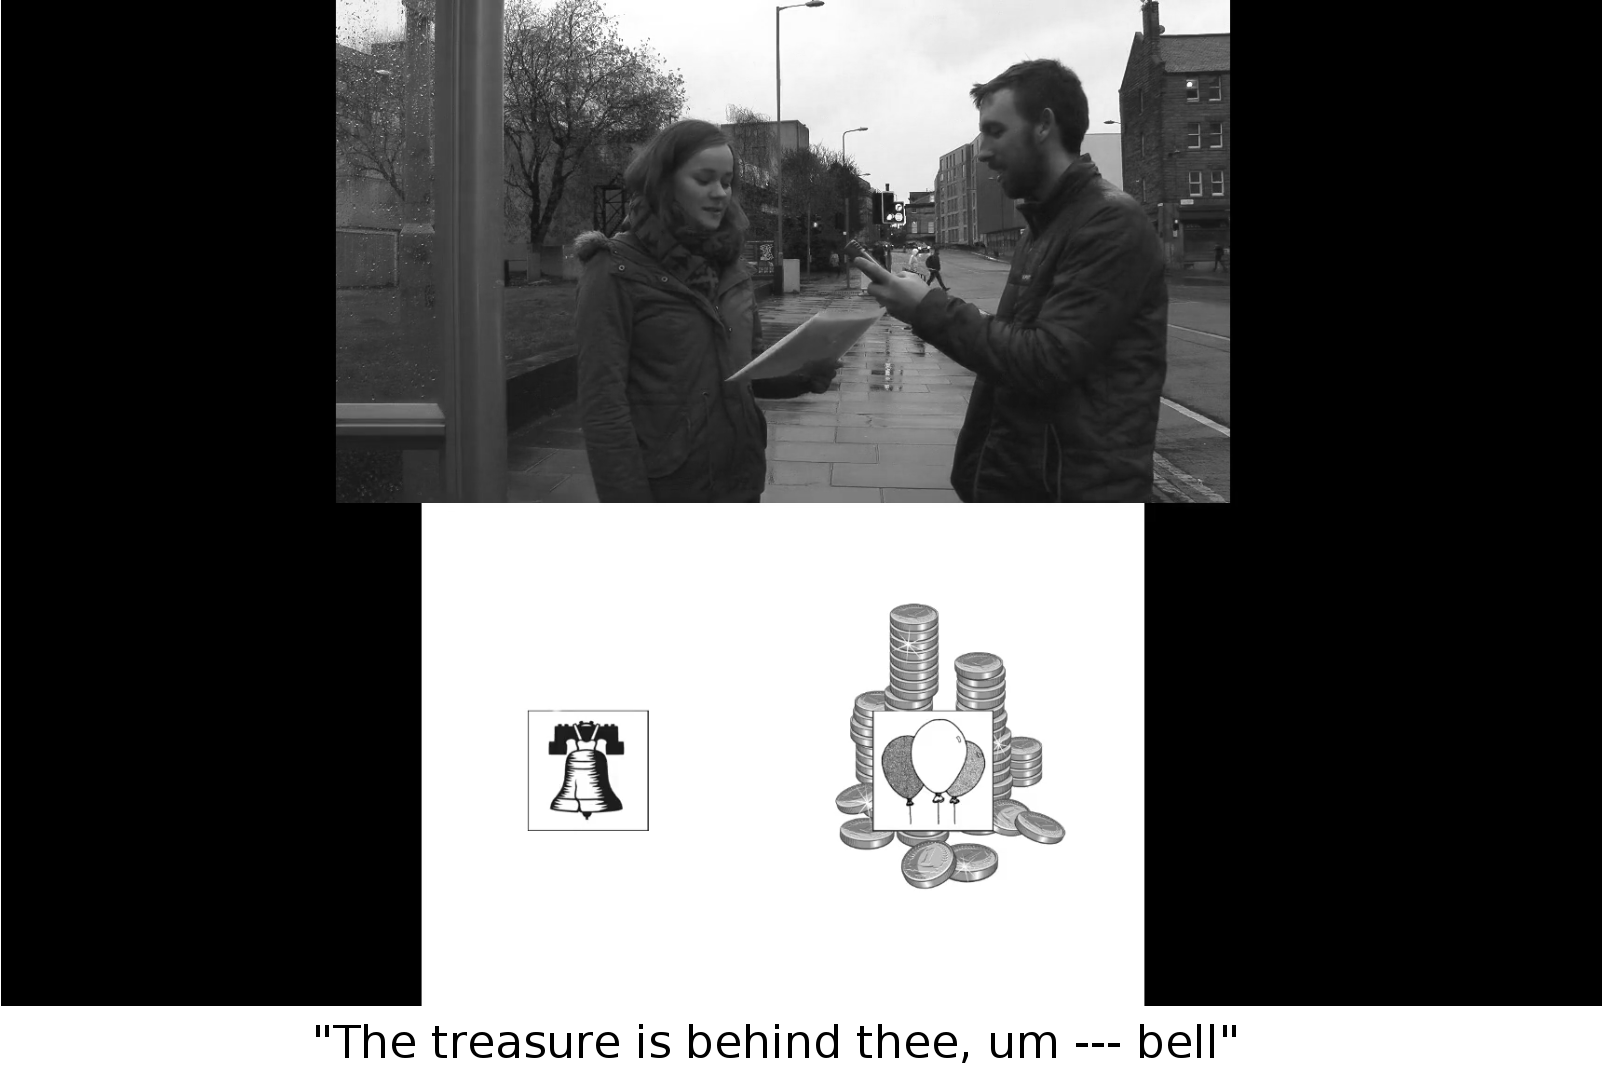
\includegraphics[scale=.2]{convincer.png}
  \caption{Screenshot of video presented to participants as an example of speaker producing utterances in a noisy environment. Screenshot shows an example of speaker producing a disfluent and dishonest utterance.}
  \label{fig:vid}
\end{figure}


To ensure that analysis could be run only on data from participants for whom the cover story held, a post-test questionnaire assessed whether participants thought it believable that the utterances were produced naturally and in the suggested context. 
This was double-checked by verbal questioning after participants were debriefed about the true nature of the experiment, by asking whether it occurred to them during the experiment that the recordings might not have been produced outside in the street.


\subsection{Procedure}
Stimuli were displayed on a 21'' CRT monitor, placed 850mm from an Eyelink 1000 Tower-mounted eye-tracker which tracked eye-movements at 500Hz (right-eye only). 
Audio was presented in stereo from speakers either side of the monitor. 
Mouse coordinates were sampled at 50Hz. 
The experiment was presented using OpenSesame version 3.0 \citep{Mathot2012}.


%\subsubsection{trial structure}
Participants were told they would see two objects and hear a speaker identify one of them as hiding the treasure. 
They were told that the objective of the game was to accrue treasure by successfully locating the treasure, the location of which the speaker would lie half the time about. Participants' instructions were to click on the object which \textit{they believed} the treasure to be behind. 
Once participants had read the instructions, the eye-tracker was calibrated.
Calibration was monitored throughout, with the experiment being paused for recalibration if the experimenter deemed it necessary.
To maintain accuracy, between each trial participants underwent a drift correction using a central fixation point, which changed from grey to red (for 500ms) upon successful fixation, signifying the start of the subsequent trial. 
Each trial began with the presentation of the two images (referent and distractor) in positions vertically central and horizontally to the left and right of centre (referents were presented equally often on each side). 
Simultaneous with presentation of the visual display was the onset of the ambient traffic audio file. 
After 1500ms, the mouse pointer appeared centrally, and the playback of the utterance began. 
Upon clicking an object, the stimuli disappeared and were replaced by the grey fixation dot, signifying progression to the subsequent trial. 
Each trial had an automatic time-out of 5000ms from utterance onset, in case participants did not click on an object.


%\subsubsection{bonus rounds}
To maintain motivation throughout the study, participants were told that there were a number of ``hidden bonus rounds'' which offered more treasure. 
Of the filler trials, 25\% did not immediately progress to the subsequent trial, instead giving a positive feedback message (regardless of which object was clicked) stating successful completion of a bonus round. 
Furthermore, participants were told that top scorers of the game would be able to enter their name on a highscore table, which was shown at the beginning of the experiment. 
Participants completed five practice trials (one of which was presented as a bonus round) prior to the main experiment. 
Eye-movements, mouse co-ordinates and object-clicked (referent or distractor) were recorded for each experimental trial.


\section{Results}
\subsection{Exclusion criteria}
For a final sample of 24, we were required to run the experient with 37 participants, recruited from the University of Edinburgh community, who participated in return for £4 remuneration. 
The data from 12 participants was excluded on the basis that they indicated either in the questionnaire (ten) or verbally (two) that they did not believe the cover story. 
Additionally, the study reported that one participant for whom the deception held had previously participated in \citet{Loy2016}, and thus they were also exlcuded. 
Analysis was run on the data from the remaining 24 participants.


\subsection{Analysis}
Analysis was carried out in R version 3.3.0 \citep{rbase}, using the lme4 package \citep{lme4}. 
Trials in which participants did not click on either the referent or distractor (0.01\%) were excluded from all analyses. 
Object-clicked (referent or distractor) was modelled using mixed effect logistic regression, testing for main effects of manner of delivery, presence of plausible speaker distraction, and their interaction as fixed effects, and including random slopes for these same variables, plus random intercepts and slopes by both subject and referent.


Eye-tracking fixation data was averaged into 20ms bins (of 10 samples) prior to analysis, and coded in terms of the area of interest (AOI), which were referent; distractor and neither image. 
The proportion of fixations to either object from the total sum of fixations was computed for each time bin. 
Mouse-tracking analysis only looked at the $X$-coordinates of the cursor.
Distance traveled by the cursor (pixels) was computed for each 20ms bin, coded for direction relative to either object. 
The cumulative mouse distance traveled toward either object in each trial was calculated by summing the distance travelled up to each time bin, and proportion of movement was calculated by taking the distance travelled toward an object, divided by the total distance travelled in that trial in either direction. 
Trials for which the total mouse distance travelled post referent-onset was less than 1/3 of the distance from the screen centre to the near edge of an object were excluded (0.03\% of trials), on the basis that it was indicative of participants' having decided prior to referent-onset upon which object to click. 
Movements beyond the outer edge of either object were excluded on the basis that it indicated `overshooting' with the cursor.


Analyses for both eye- and mouse-movements were conducted over a time window from referent onset to 800ms post-onset. 
This window matches that of \citet{Loy2016}, based on evidence that reference is established in eye-movements around the 400-800ms post noun-onset mark \citep{Eberhard1995}, and covering the duration of the longest critical referent (776ms). 
Models of eye-movements used the empirical logit transform of fixations to the referent minus the empirical logit transform of fixations to the distractor \citep{Barr2008}.
Mouse-movements were modelled analogously. 
This allowed us to model the eye- and mouse-movement bias towards either object over the other: A value of zero indicated no bias towards either object, and positive and negative values indicated a bias towards the referent and distractor respectively. 
Models included fixed effects of time (Z-scored), delivery (fluent or disfluent) and speaker distraction (absent or present), and all interactions. 
Random intercepts and random slopes for time, delivery and distraction were included for both subjects and items.


\subsection{Final object-click}
Responses show the same overall tendency to interpret an utterance as truthful as was found in \citet{Loy2016}, with 57\% of trials resulting in a click on the referent and only 43\% on the distractor. 
Table \ref{table:objctclck} shows the percentage of mouse-clicks on each object by condition.
A logit regression model of object-clicks showed that participants were less likely to click on the referent following a disfluent utterance than a fluent one ($\beta = -2.24,SE = 0.67,p<.001.$). 
This is in keeping with the literature \citep{Brennan1995, Swerts2005} and with the results of \citet{Loy2016}: Manner of delivery influences participants' global interpretations of the speaker's truthfulness. 
The presence of a plausible speaker distraction was not found to affect responses; neither was the interaction between delivery and distraction. 
The bias toward interpreting disfluency as a sign of dishonesty appeared to be explicit for 19 out 24 participants, as indicated in the post-test questionnaire. 
Table \ref{table:objctclck} shows the percentage of mouse-clicks on each object by condition.


\begin{table}[ht]
\centering
\begin{tabular}{rrrrrr}
  \hline
& \textbf{Delivery} & Disfluent & Disfluent & Fluent & Fluent \\ 
& \textbf{Speaker-distraction} & Absent & Present & Absent & Present \\
  \hline
Distractor & &  62\% &  62\% &  23\% &  24\% \\ 
  Referent & &  38\% &  38\% &  77\% &  76\% \\ 
   \hline
\end{tabular}
\caption{Mouse clicks on each object by condition.}
\label{table:objctclck}
\end{table}

\subsection{Eye-movements}
The time-course (referent onset to 2000ms post-onset) of fixations to referent and distractor can be seen for the fluent conditions (Fig. \ref{fig:flueye}) and the disfluent conditions (Fig. \ref{fig:diseye}). 
Visualisation of the time-course of fixations show that for fluent utterances, participants displayed an early fixation bias towards the referent, which began to present itself prior to mean critical noun offset. 
For disfluent utterances, the picture is more complex---whilst a fixation bias towards the distractor over the referent was present, this only appeared later on in the trial.
When an alternative, local cause of disfluency (the car-horn) was present prior to a disfluency, participants showed a tendency to initially fixate towards the referent, before the later bias towards the distractor. 
This initial fixation bias to the referent was not apparent when the car-horn was absent.


\begin{figure}[Ht]
  \centering
	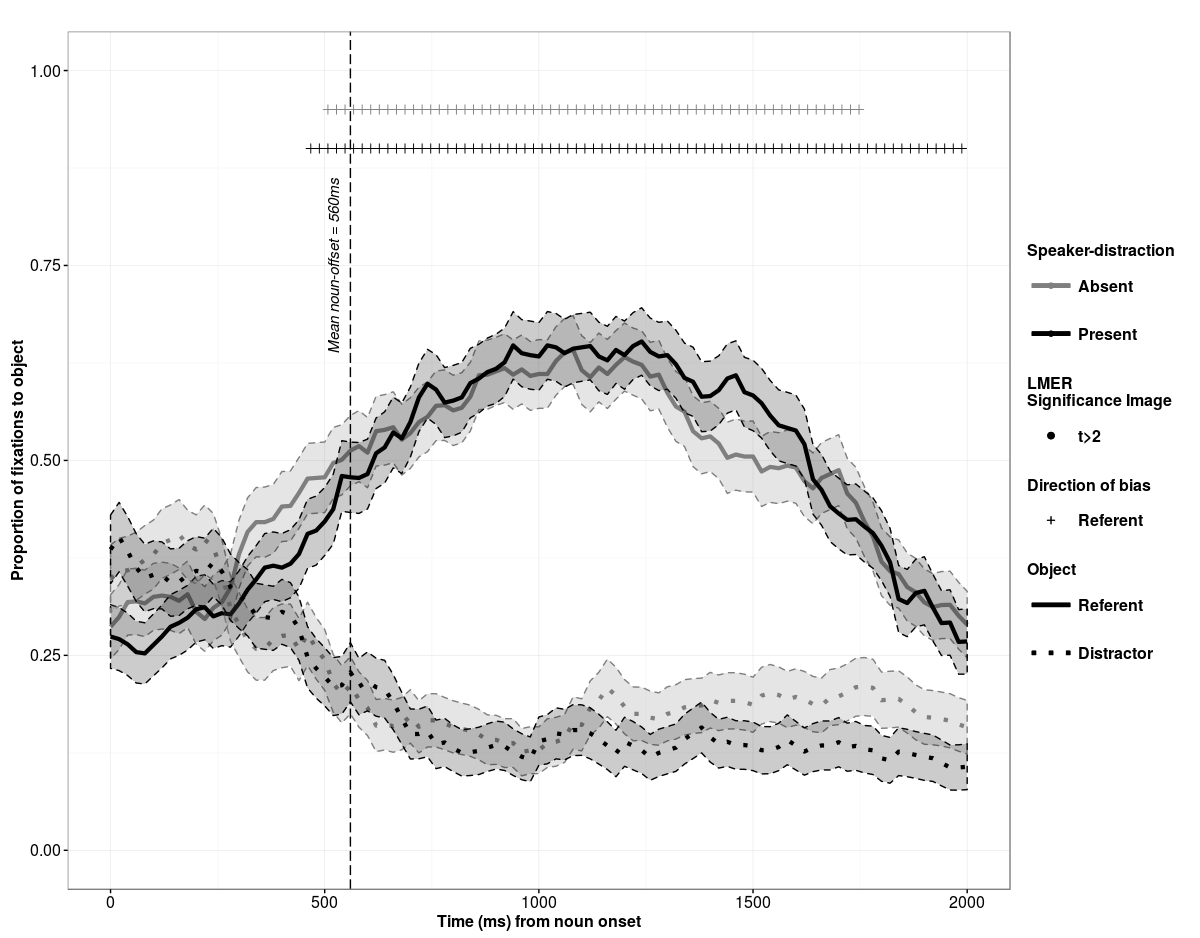
\includegraphics[scale=.5]{fluent.png}
  \caption{Mean proportion of fixations to either object (referent and distractor) for fluent utterances split by presence of speaker distraction, calculated out of the total sum of fixations for each 20ms time bin from referent-onset to 2000ms post-onset. Shaded areas represent $\pm 1$ standard error of the mean. Time bins in which a bias towards either the referent or distractor was evident are highlighted with respect to condition and direction of bias (assessed by a mixed effect model estimating the empirical logit of fixations to the referent minus the empirical logit of fixations to the distractor, with by-subject and by-item random intercepts).}
  \label{fig:flueye}
\end{figure}


\begin{figure}[Ht] % might need to change placement
  \centering
	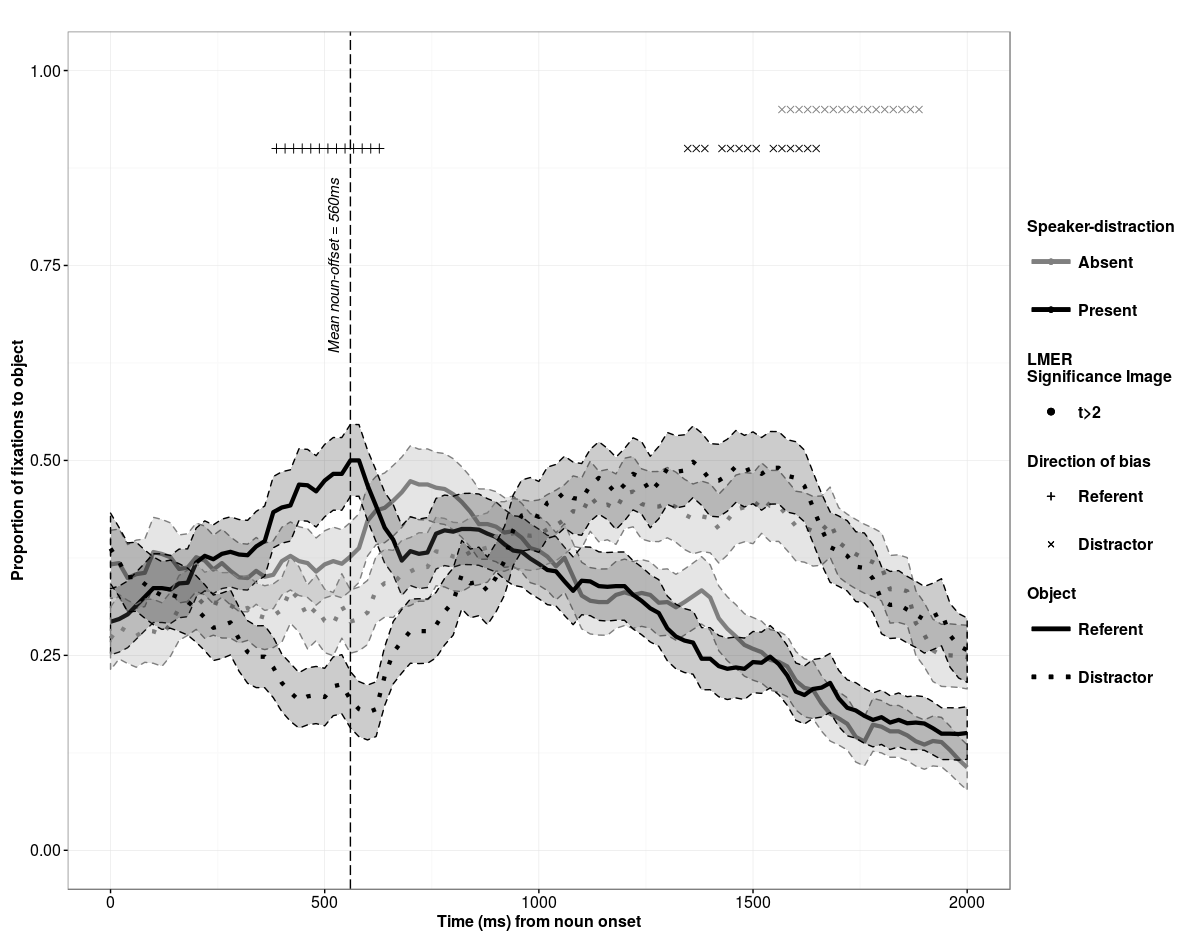
\includegraphics[scale=.5]{disfluent.png}
  \caption{Mean proportion of fixations to either object (referent and distractor) for disfluent utterances split by presence of speaker distraction, calculated out of the total sum of fixations for each 20ms time bin from referent-onset to 2000ms post-onset. Shaded areas represent $\pm 1$ standard error of the mean. Time bins in which a bias towards either the referent or distractor was evident are highlighted with respect to condition and direction of bias (assessed by a mixed effect model estimating the empirical logit of fixations to the referent minus the empirical logit of fixations to the distractor, with by-subject and by-item random intercepts).}
  \label{fig:diseye}
\end{figure}


Analysis of the window from referent-onset to 800ms post-onset confirmed what is evident from visualising the time-course of fixations. 
When presented with a fluent utterance, participants' fixations toward the referent over the distractor increased over time ($\beta = 0.64, SE = 0.12, t=5.44.$). 
In contrast, this fixation bias was reduced when the delivery was disfluent ($\beta = -0.60, SE = 0.06, t=-10.62.$). 
For disfluent utterances, when the car-horn was present prior to disfluency (providing an alternative explanation of the disfluency), participants' fixations towards the referent over time increased in contrast to when the car-horn was absent ($\beta = 0.18, SE = 0.08, t=2.20.$). 
The presence of the car-horn was not found to have an effect on the tendency to fixate on the referent for fluent utterances ($t=-0.7.$).


\subsection{Mouse-movements}
The proportion of mouse-movements (distance traveled) towards either object was computed for each 20ms bin from referent onset to 2000ms post-onset. 
Figures \ref{fig:mflu} and \ref{fig:mdis} and show the proportion of mouse-movements towards either object in fluent and disfluent conditions respectively. 
Analysis of the window from referent-onset to 800ms post-onset patterned with the eye-tracking data. 
When presented with a fluent utterance, participants' movements to the referent over the distractor increased over time ($\beta = 0.49, SE = 0.07, t=7.36.$). 
This movement bias towards the referent over the distractor decreased when the delivery was disfluent ($\beta = -0.64, SE = 0.04, t=-16.71.$). 
When the car-horn was present prior to a disfluency, participants' tendency to move towards the referent over the distractor increased in comparison to a disfluency not preceded by the car-horn ($\beta = 0.37, SE = 0.05, t=6.73.$).


\begin{figure}[Ht]
  \centering
	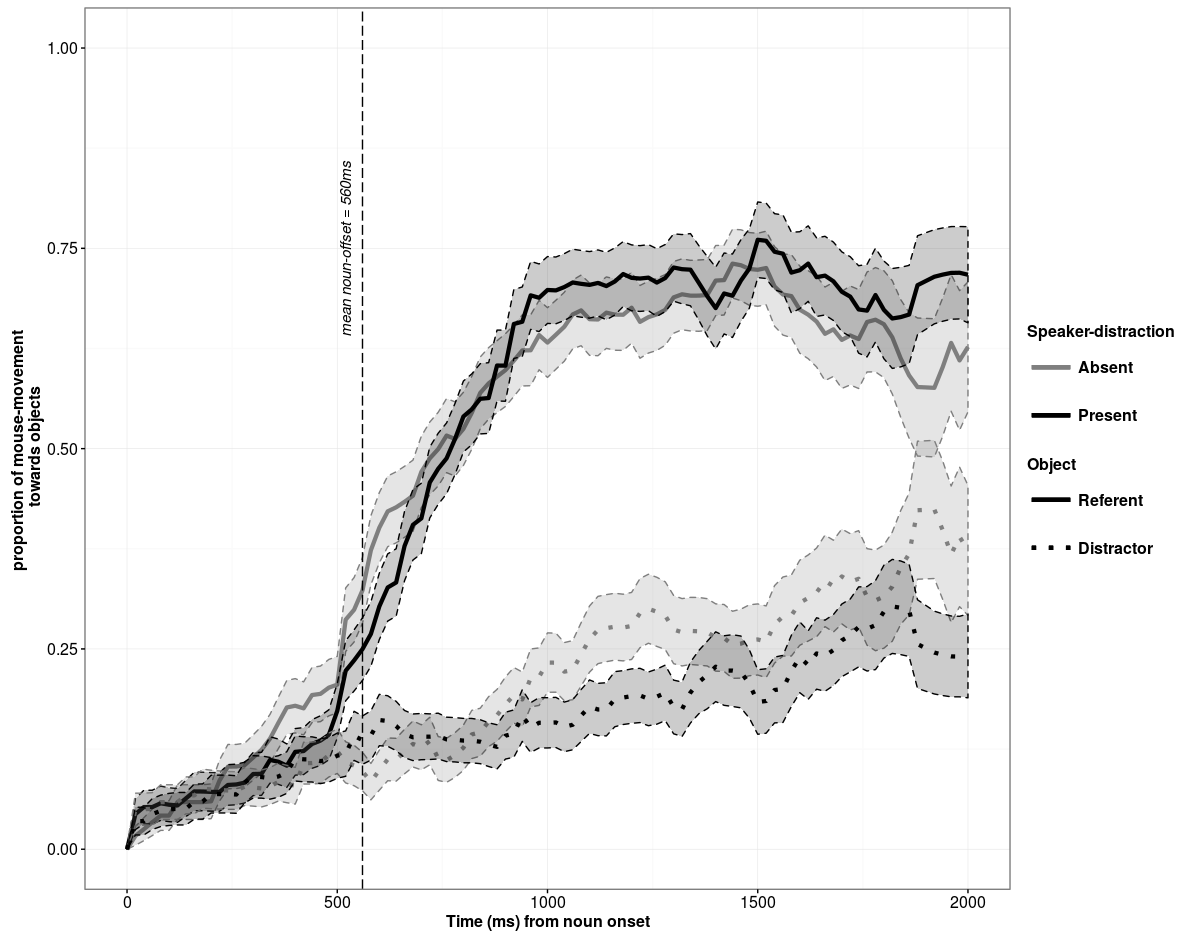
\includegraphics[scale=.5]{mflu.png}
  \caption{Mean proportion of cumulative distance traveled toward each object (referent or distractor) in fluent conditions split by presence of speaker distraction, from referent onset to 2000ms post-onset. Proportions calculated out of total cumulative distance moved the mouse from referent-onset until that time bin. Shaded areas represent $\pm 1$ standard error of the mean.}
  \label{fig:mflu}
\end{figure}


\begin{figure}[Ht]
  \centering
	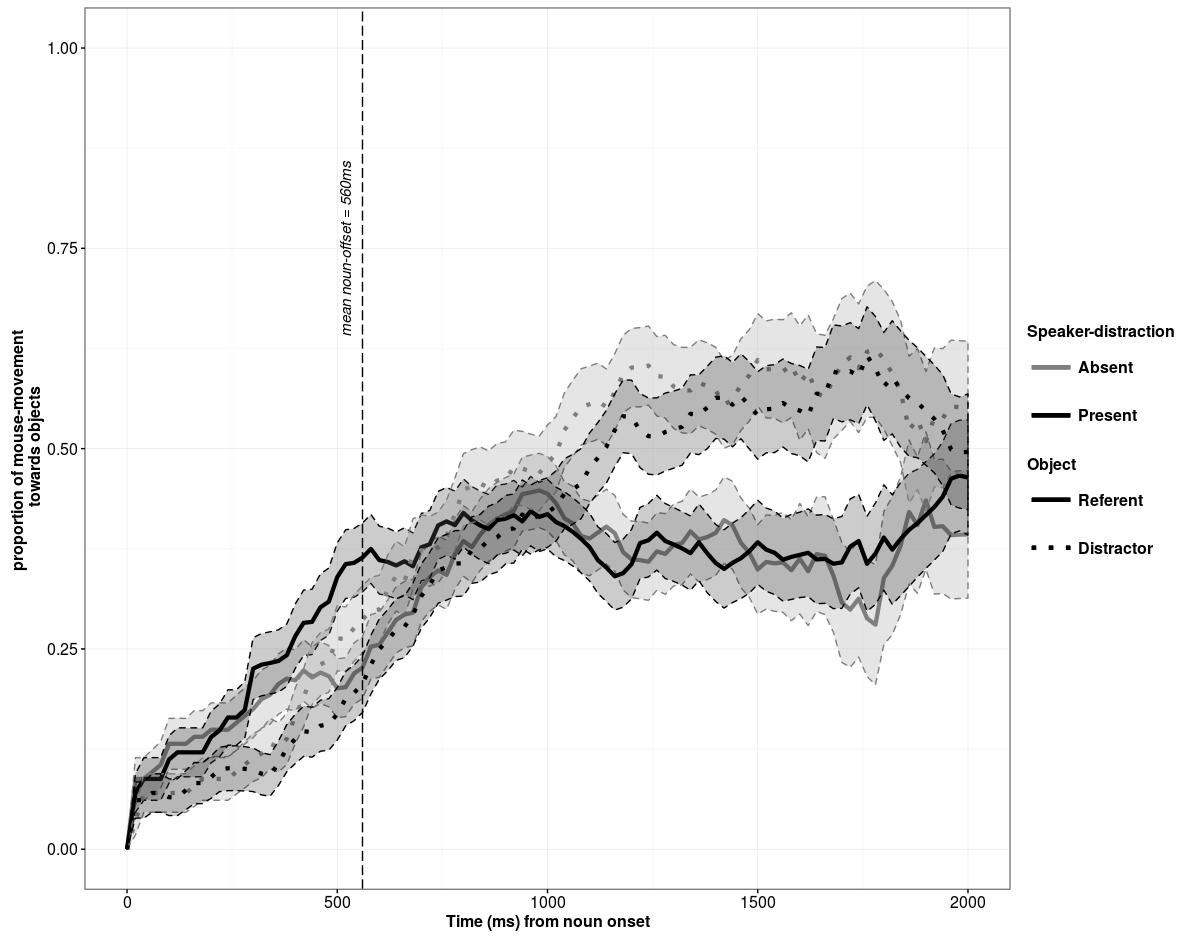
\includegraphics[scale=.5]{mdisfl.png}
  \caption{Mean proportion of cumulative distance traveled toward each object (referent or distractor) in disfluent conditions split by presence of speaker distraction, from referent onset to 2000ms post-onset. Proportions calculated out of total cumulative distance moved the mouse from referent-onset until that time bin. Shaded areas represent $\pm 1$ standard error of the mean.}
  \label{fig:mdis}
\end{figure}


\section{Discussion}
Listeners' pragamatic judgments about a speaker's honesty were effected by manner of delivery.
In keeping with the literature on deception perception, participants associated speaker disfluency with lying \citep{Zuckerman1981,depaulo2003cues}. 
As shown in \citet{Loy2016}, listeners made these judgments quickly: 
The effect emerged at an early stage in utterance processing, with eye- and mouse-tracking data showing biases towards referent and distractor for fluent and disfluent utterances respectively.
Additionally, the effect was showed that the disfluency-lying association is robust against the presentation of speech in a noisy environment, in which there are potential distractions for the listener. 


The availability of an alternative, utterance-local cause of disfluency (the speaker being momentarily distracted by a car-horn) was used to investigate whether listeners' association between disfluency and lying are heuristically calculated, or whether they involve reasoning about the speaker's production system. 
Participants showed an increase in eye- and mouse- movements to the distractor when presented with disfluent utterances---indicating the emergent bias towards interpreting the utterance as dishonest. 
Critically, in situations when the disfluency could have been caused by a car-horn, this was preceded by an initial tendency to fixate and move towards the referent, only later fixating on and selecting the distractor. 
The fact that the car-horn provided a local cause of disfluency is important here, as its influence shows that the associations which participants had between disfluency and lying was sensitive to contextual information which only occurred during speech. 
This could suggest that listeners momentarily model the speaker in order to attribute a cause to a particular disfluency. 


This account of this suggests that participants made early inferences about the cause of a given disfluency.
This reasoning took into account contextual information about what might cause disfluency for a given speaker.
Eventually, however, this was overridden by the association between disfluency and lying.
On this view, listeners appear able to dynamically reason about the most likely explanation of disfluency, and, as the speech unfolds, make attributions about why a particular speaker in a particular context was disfluent. 
This is in line with the speaker modelling account found in lying research, suggesting that listeners detect deception by reasoning about cues relating to the cognitive load of the speaker\citep{Zuckerman1981,depaulo2003cues}.
For the speaker modelling view, the findings here---a local cause of disfluency modulating listeners' disfluency-lying assocation---suggest that, if speaker modelling occurs, then it does so actively, during the early stages of comprehension. 


However, our findings are not incompatible with an explanation in terms of listeners simply having direct associations between disfluencies and certain properties of language use such as lying. 
If Listeners heuristically associate disfluency and lying, to account for the findings here, such an heuristic would simply have to be sensitive to any loud noises which precede a disfluency.
Importantly, disfluency effects on comprehension could still be an heuristically calculated response, rather than the result of reasoning about the production system of a particular speaker.
It is unclear, however, how such a view would account for listeners deciding what constitutes as potentially distracting for a speaker. 
For instance, would listeners discern between the car-horn used here, which was situated within the context of the speaker's environment, and a similarly loud noise occurring outside of the recording? 
Reasoning about what is distracting for a given speaker is essentially equivalent to a speaker modelling account. 


A remaining question is how to fit the current study in with the account given in \citet{Arnold2007}, in which contextual effects on disfluency biases were limited to more global factors which would affect the speaker throughout a discourse, and in which listeners were not sensitive to local causes of disfluency.
There are certain differences between \citeauthor{Arnold2007}'s Experiment~3 and the one described here which might explain the contrary findings.
Firstly, it could be that believable sounding disfluencies as-caused-by distraction are hard to construct:
In the experiment here, the distracting noise overlapped the onset of the critical disfluency \spex{Thee---uh---}, whereas in \citeauthor{Arnold2007}'s study it did not.
%intuitively, the elongated 'thee' coming after the car-horn would sound weird. 

%I can't really think of any thing else which might explain why ours found something and arnold's did not. The other day you mentioned something about ours being pragmatics and Arnold's more predictions about semantic content. I can't see how this might explain it? 

Utterance-local contextual information influenced listeners' moment-to-moment pragmatic inferences about disfluencies. 
Whilst being eventually overridden by listeners' biases towards interpreting disfluent utterances at dishonest, the availability of an alternative, external cause of speaker disfluency (being momentarily distracted) resulted in an initial bias in eye- and mouse-movements towards the referent. 
This contextual effect could be explained in terms of heuristically calculated assocations between disfluency and lying and between disfluency and loud noises.
It is not clear, however, whether, nor how, listeners might judge what constitutes as potentially distracting for a speaker.
Alternatively, these findings could suggest that participants made early inferences about the potential causes of a specific disfluency, actively modelling the speaker's production system during the online processing of speech, and in line with previous accounts of deception detection. 



\bibliography{e2}

\end{document}
%%% Local Variables:
%%% mode: latex
%%% TeX-master: t
%%% End: